%
% File hicss51.tex
%
% Contact: Holm Smidt, hsmidt@hawaii.edu
%%
%%
%% Based on the style files for ACL 2015 by 
%% car@ir.hit.edu.cn, gdzhou@suda.edu.cn


\documentclass[10pt]{article}
\usepackage[T1]{fontenc}
\usepackage[latin1]{inputenc}
\usepackage[table]{xcolor} 
\usepackage[letterpaper]{geometry}
\usepackage{hicss51}
\usepackage{times}
\usepackage[none]{hyphenat}
\usepackage{url}
\usepackage{latexsym}
\usepackage{minted}
\usepackage{graphicx}
\graphicspath{{images/}}

\newcommand{\sansserifformat}[1]{\fontfamily{cmss}{ #1}}%

%\setlength\titlebox{5cm}

% You can expand the titlebox if you need extra space
% to show all the authors. Please do not make the titlebox
% smaller than 5cm (the original size).


\title{An Explicative and Predictive Study of Employee Attrition}

\author{Nesreen El-rayes\\
  MTSM at NJIT \\
  {\underline{nde4@njit.edu}} \\\And
  Michael Smith\\
  MTSM at NJIT \\
  {\underline{mes6@njit.edu}}\\\And 
  Stephen Taylor\\
  MTSM at NJIT \\
  {\underline{smt@njit.edu} (Corr. Auth.)} \\}

\date{}

\begin{document}
\maketitle
\begin{abstract}
WRITE THIS IN THE END
\end{abstract}

\section{Introduction}
Building and maintaining a stable, productive, collaborative, and high-quality workforce is a primary concern 
for the majority of managing principals as success in this area tends to be a key factor contributing the 
overall firm prosperity [CITATIONS??].  Inevitably, all firms will experience employee attrition.  
Involuntary attrition is often the result of profitability and performance pressures, department or business 
line obsolescence, and mergers and acquisitions, among other factors [CITATIONS??].  In contrast,
voluntary attrition is driven predominately by employee concerns [CITATIONS].  Such considerations 
my focussed around, but not limited to, managerial direction, compensation and benefits, firm culture, 
firm desirability and location, promotion potential as well as non firm specific motivations, e.g. medical 
conditions or retirement. 
  
A central objective of the majority of human resource departments is to understand the root causes 
behind voluntary employee attrition and develop an associated mitigation strategy.  Effectively 
navigating such issues generally resulted in explicit positive monetary effects stemming from increased 
firm revenue and cost reductions manifested through the work retained highly performant employees. 
In addition, identifying and resolving issues found to be common to employee attrition often implicitly 
enhances firm culture and workplace desirably which in turn enables the recruitment of higher quality 
staff which further improve retention, firm operation, and business practices.  
We feel that the compounding effect nature of 
this employee attrition feedback loop on the overall success or failure of the firm is the essential motive 
for conducting a through investigation into this matter. [MORE CITATIONS FOR THIS PARAGRAPH]  

Traditionally, employee attrition and retention issues tend to examined through qualitative and anecdotal 
measures.  Specifically, human resources staff tend to conduct exit interviews after an employee provides 
a resignation notice in order to ascertain the motivations behind the decision to leave.  Although 
these conversations may be direct and candid, i.e. in the event an employee is leaving for a significantly 
more senior role or needs to change geographic location for family reasons, in actuality, human resources staff
encounter considerable difficulty discerning the employee's actual rationale.  By way of example, employees 
seldom offer negative criticism of management during exit interviews for fear of future personal retribution 
or inadvertent retaliation towards their close colleagues who will still remain at the firm.
These circumstances impact the employee attrition data aggregation and quality assurance process 
by making it cumbersome, at a minimum, which leads to additional difficulties determining which 
attrition issues should be of primary importance for management to resolve. In addition, employee 
attrition data is typically high confidential and only accessible to key stakeholders internally 
within a firm.  This fact has been a major impediment for the progression of academic research on 
this topic. [CITATIONS] 

Recently, internet based platforms such as GlassDoor and LinkedIn oriented towards working 
professionals have amassed large quantities of publicly available information related to individual 
employee resumes including employment history, frank reviews of firm culture, desirability, and management
as well as anonymous feedback.  Although this data often lacks attritional motivation information at 
the individual employee level, when combined with aggregate firm culture and management rankings, 
one may glean a number of insights into the collective behavior and motivations behind individual 
decisions to transition to a new employer. Our major aim is precisely in this vein.  More specifically, 
we conduct a quantitative data analysis of employee attrition motivations as well as develop 
predictive models that will enable human resources staff identify employees whose firm separation 
may be imminent.

We extend the work of \cite{Smart2016} who examine employee attrition and retention issues based upon 
a collection of approximately five thousand anonymously submitted resumes to Glassdoor.  We provide 
SUMMARY OF DATA ANLAYSIS EXTENSIONS.  In addition, SUMMARY OF NEW MODELS. Lastly, we delineate 
future data acquisition, analysis and model development extensions that we seek to investigate 
in future work. 

This article is organized as follows ... TYPE WHEN FINISHED 

\section{Data Description and Feature Engineering}

We first turn to describing the content extracted from a collection of 
employee resumes that will form the basis for the subsequent attrition studies. 
Next, we provide a variety of summary statistics of this information that 
are relevant for the design of latter predictive models.  Then we discuss 
our data normalization process and 
several features constructed from this original data which will be utilized 
as input into these models.
In addition, we outline limitations of this dataset and ideas for improvement  
in future work.

\subsection{Data Source Description}\label{datdes}

We worked in conjunction with the authors of \cite{Smart2016} to obtain 
a collection of 5550 examples of employee job transitions between 
2007 and 2016 which were sourced from an extensive proprietary database of 
resumes shared anonymously though Glassdoor's platform.  A job transition 
is define to be any instance of an employee listing a new role on their 
resume which may be associated with the present or original or a new employer
designated as internal and external moves.  Internal moves are typically 
significant in the sense of the employee either changing roles or 
being promoted within an organization as opposed to being reassigned 
within a current team. External moves are of interest for our 
attrition studies as in this situation employees leave their original 
firm entirely.

We summarize several salient features of the dataset construction process 
and expound upon details relevant to model development below; we refer the
reader to \cite{Smart2016} for a complete description of the data source. 

Each employ job transition contains 45 attributes.  Relevant attributes 
include employee specific information. Namely, a binary identifier 
indicating if the employee remained within or left their original firm,
the start and end dates of employment at the original firm, the 
employee's average salary during their tenure with the original employer, 
and the employee's job title. 
In addition, each transition includes employer related information. 
Specifically, employer name and metro location, the industry sector of which the employer 
is a member, the founding year of the firm, and the total number of employees. 
Finally, employer rating information is included.  Particular ratings are 
given for the following GlassDoor created categories: overall, firm CEO, friend recommendation 
business outlook, career opportunities, compensation and benefits, culture and values, 
worklife balance, and senior management. 
We note that in the event the employee transitioned to a new firm, when applicable,
the above information specific to both the original and new employer is present in this dataset. 
Finally, this dataset if fully populated with the exception of missing values in 
approximate 6\% of the original and new employer founding year values, respectively;
such null values are disregarded 
only in studies that depend upon this variable below.

\subsection{Summary Statistics, Feature Engineering and Data Normalization}

First, several summary statistics are presented in order to outline 
the main content of the dataset that will be further explored below.
Next, we discuss our feature construction process to build variables 
that will be important to latter exploratory studies and predictive 
model design.  Finally, we describe the quantile normalization process 
we use in order to ensure all variables are on the same scale prior 
to being input into the predictive models.

Of the 5550 total employee job transitions in this dataset, 
a total of 1429 employees remained at their present firm whereas a majority of 4121 
transitioned to a new firm.  This confirms a claim \cite{Smart2016} indicating 
that approximately three quarters of employees leave their employer during a job 
transition.  We now graphically summarize several distributional aspects of 
attributes associated with these transitions.

Compensation, benefits, and other forms of financial remuneration are typically play 
a critical role in an employee's job selection process.  In fact, an offer to 
substantially increase one's salary is a common impetus for a job transition. 
In the left subplot of Figure \ref{fig:avgsal}, we plot the average 
annual salary distribution 
of the employer during their tenure at their original employer over our full dataset.  
Salaries ranged from \$15,140 to \$240,000 per year.  We note that this sample 
is slightly overweight in terms of the representation of low-wage workers 
in comparison with national income distributions [CITE]. In addition, 
approximately 9\% of workers have salaries greater than \$100,000, which further 
indicates a slight low-wage bias with respect to the entire US workforce population. 
However, we note the generate shape of this distribution does indeed closely approximate 
that of the full workforce [CITE].
%
\begin{figure}[thb]
    \centering
	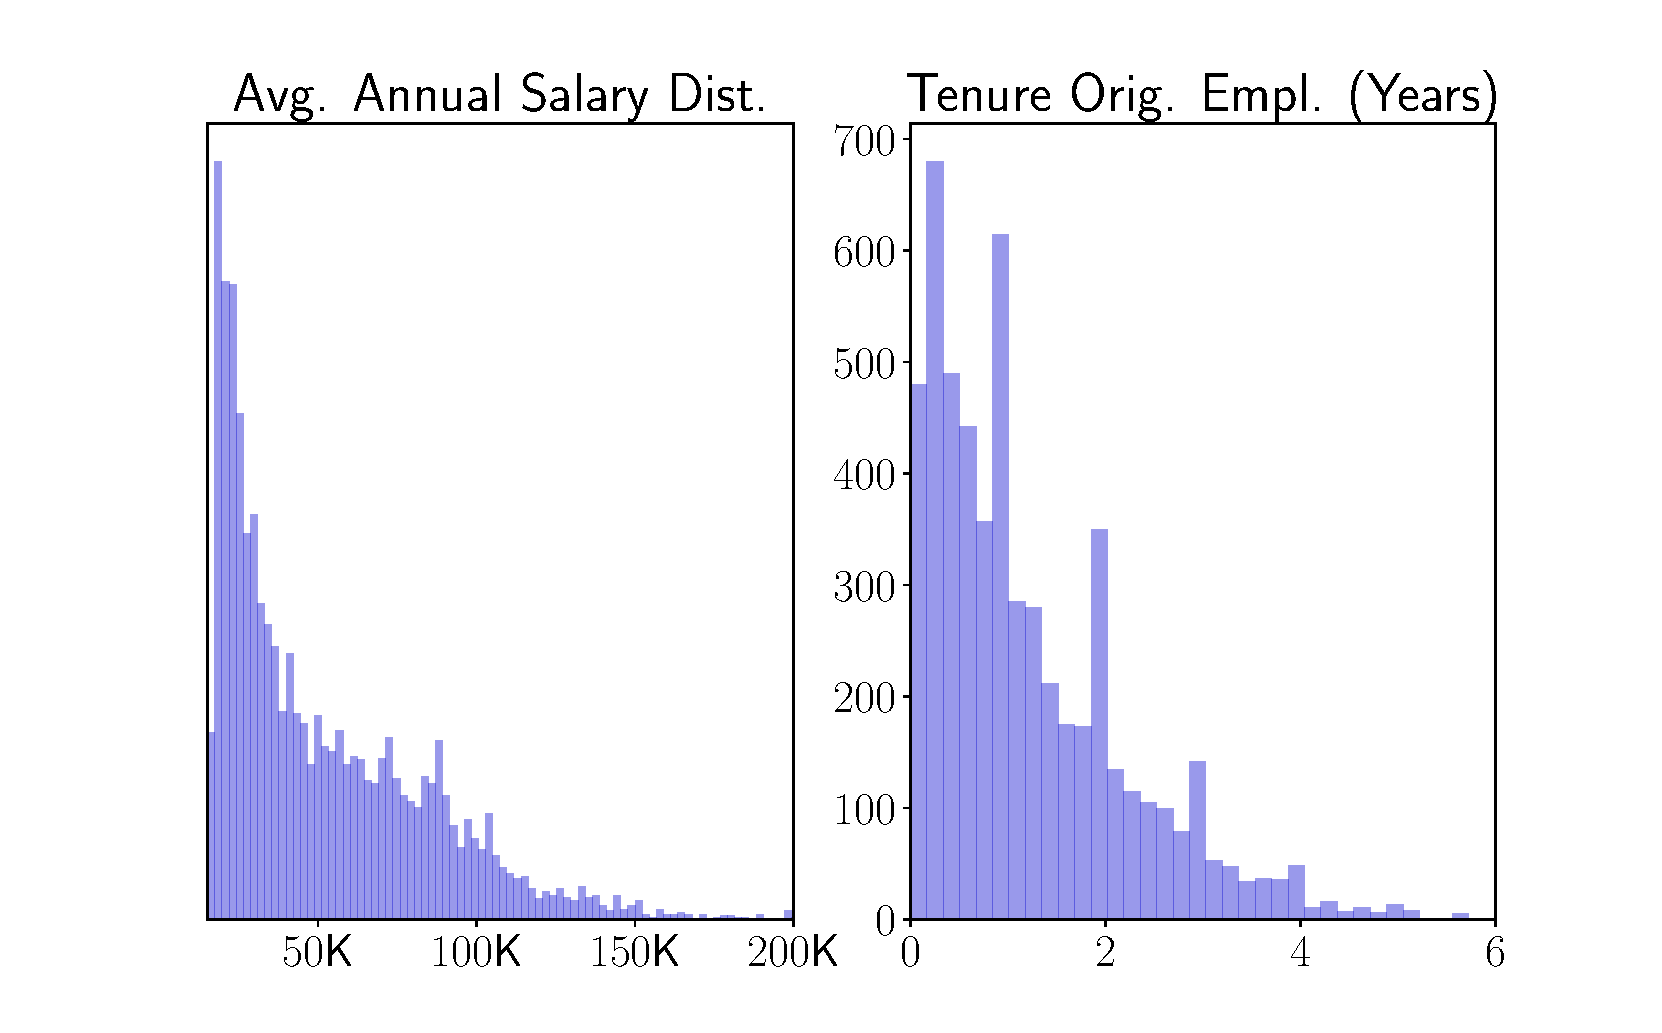
\includegraphics[width=1.0\linewidth]{avgsal.pdf}
    %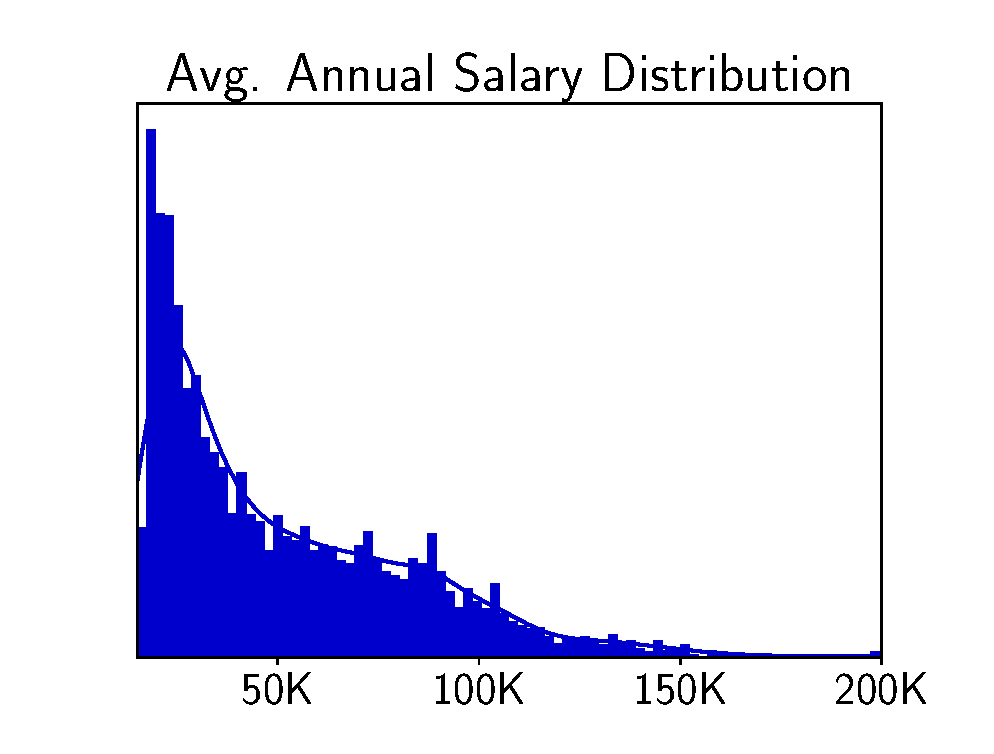
\includegraphics[trim={3cm 3cm 3cm 3cm}, clip,width=0.9\linewidth]{avgsal.eps}
	\caption{Employee average salary and tenure distribution at Original employer}
	\label{fig:avgsal}
\end{figure}
%
In the right subplot of Figure \ref{fig:avgsal}, we display the tenure of each 
employee at their original employer prior to a job transition which is similar to
summary information presented in \cite{Smart2016}. Note that overall these tenures 
are relatively short and the distribution exhibits concentrated counts near end of year 
times when performance reviews typically take place.  

Next, in table \ref{tab:indtab}, we count the industry of the original employer 
of all job transitions being considered and display all such industries exceeding 
50 such transitions.
%
\begin{table}
  \rowcolors{2}{gray!25}{white}
  \centering
  \caption{Transition Counts Per Industry}
  \begin{tabular}{cccc}
    \rowcolor{gray!50}
      Industry & Cnt. & Industry & Cnt. \\
      Retail & 1357 & Manufact. & 191\\
      Education & 766 & Insurance & 144\\
      Info. Tech. & 718 & Media & 113\\
      Finance & 590 & Acct. \& Legal & 101\\
      Bus. Services & 369 & Energy & 92\\
      Food Services & 275  & Travel & 70\\
      Telecom & 248 & Biotech & 62\\
      Health Care & 208 & Transportation & 58\\
	\label{tab:indtab}
  \end{tabular}
Original employer sector counts for industries with more than 50 job transitions.
\end{table}
%
Note that the Retail and Education industries are overrepresented which 
provides a further indication as to why lower salaries are also above those of the 
national distribution. In addition, we have sufficient data to study employee industry 
transition patters for many of the industries listed in this table which 
we explore in more detail in the subsequent section.

In Figure \ref{fig:emplstat}, we display two additional histograms related to original 
employer specific information.  In the left subplot, we present the distribution of the 
original firm's founding date.  This histogram was left truncated to begin at 1750 with a minimum 
founding date of 1625 for the City of New York.  Typically, firms with earlier founding 
dates are municipalities or governmental organizations. 
%
\begin{figure}[thb]
    \centering
	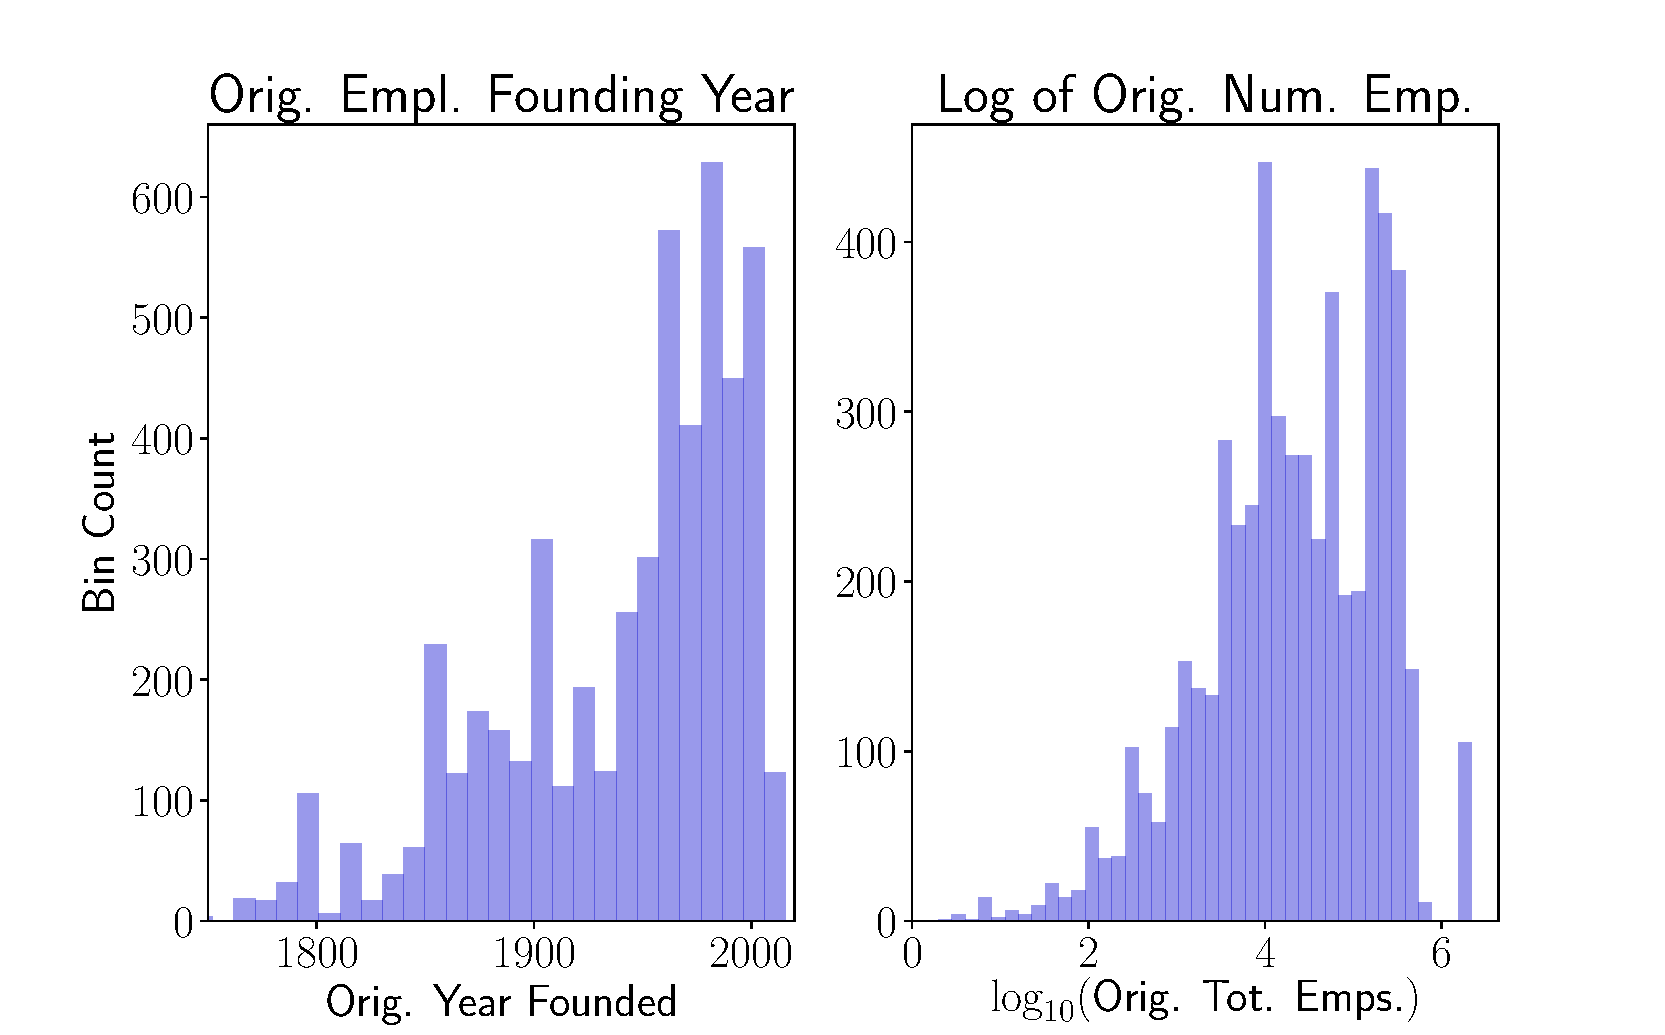
\includegraphics[width=1.0\linewidth]{emplstat.pdf}
    %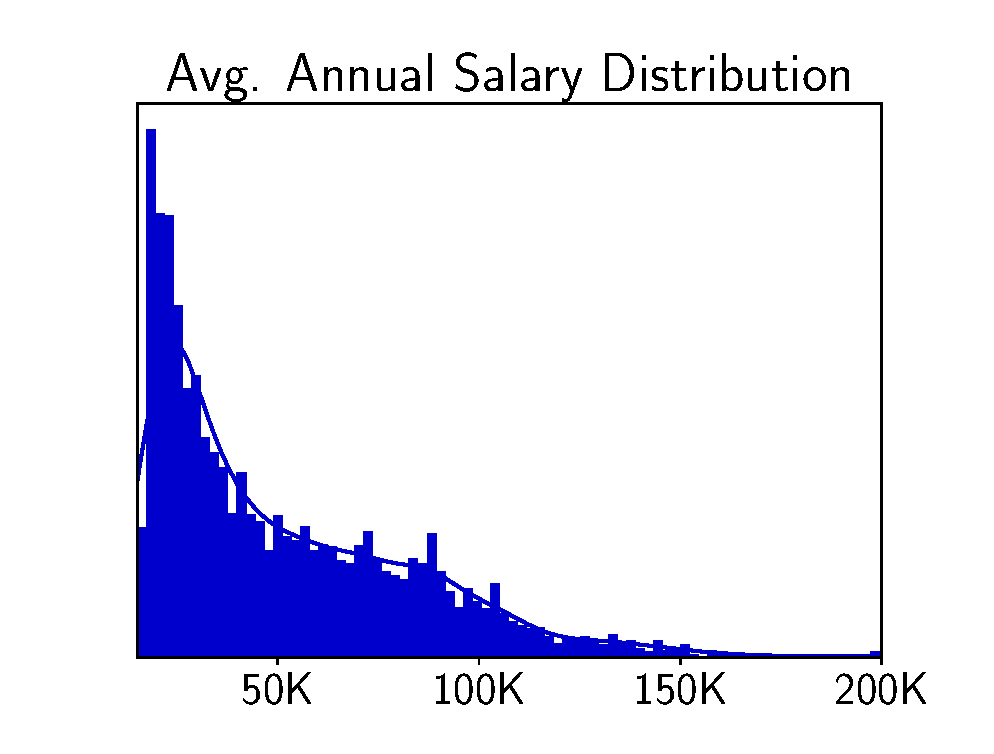
\includegraphics[trim={3cm 3cm 3cm 3cm}, clip,width=0.9\linewidth]{avgsal.eps}
	\caption{Original employer founding year and employee number distributions}
	\label{fig:emplstat}
\end{figure}
%
Note that we have an effective samplings of older and modern firms with a 
median founding date of 1962.  In addition, we consider relatively few 
firms that were founded within the past twenty years in this sample as 
indicated by the height of the final bar of the histogram.   Next, in 
the right subplot of Figure \ref{fig:emplstat}, we display the log-histogram 
of the number of employees at each original firm being considered. The majority 
of employees work at larger firms which employ between ten thousand and one million 
people.  In particular, only a small fraction of employees work at small 
firms with fewer than one hundred colleagues.  Finally, the largest employer 
is Walmart with approximately 2.2 million employees.

Next, in Figure \ref{fig:vioplt}, we display original employer violin plots of ratings data in nine 
categories which includes career opportunities, compensation and benefits, company culture, 
overall rating, senior management, work-life balance, outlook, CEO, and friend recommendation 
ratings.  Here mean values are depicted by white circles in each form whereas standard deviations 
about either side of the mean are displayed by centered black bars.  The general shape of 
each violin is determined by a symmetric display of a kernel density estimate of the 
probability distribution of each rating variable.
%
\begin{figure}[thb]
    \centering
	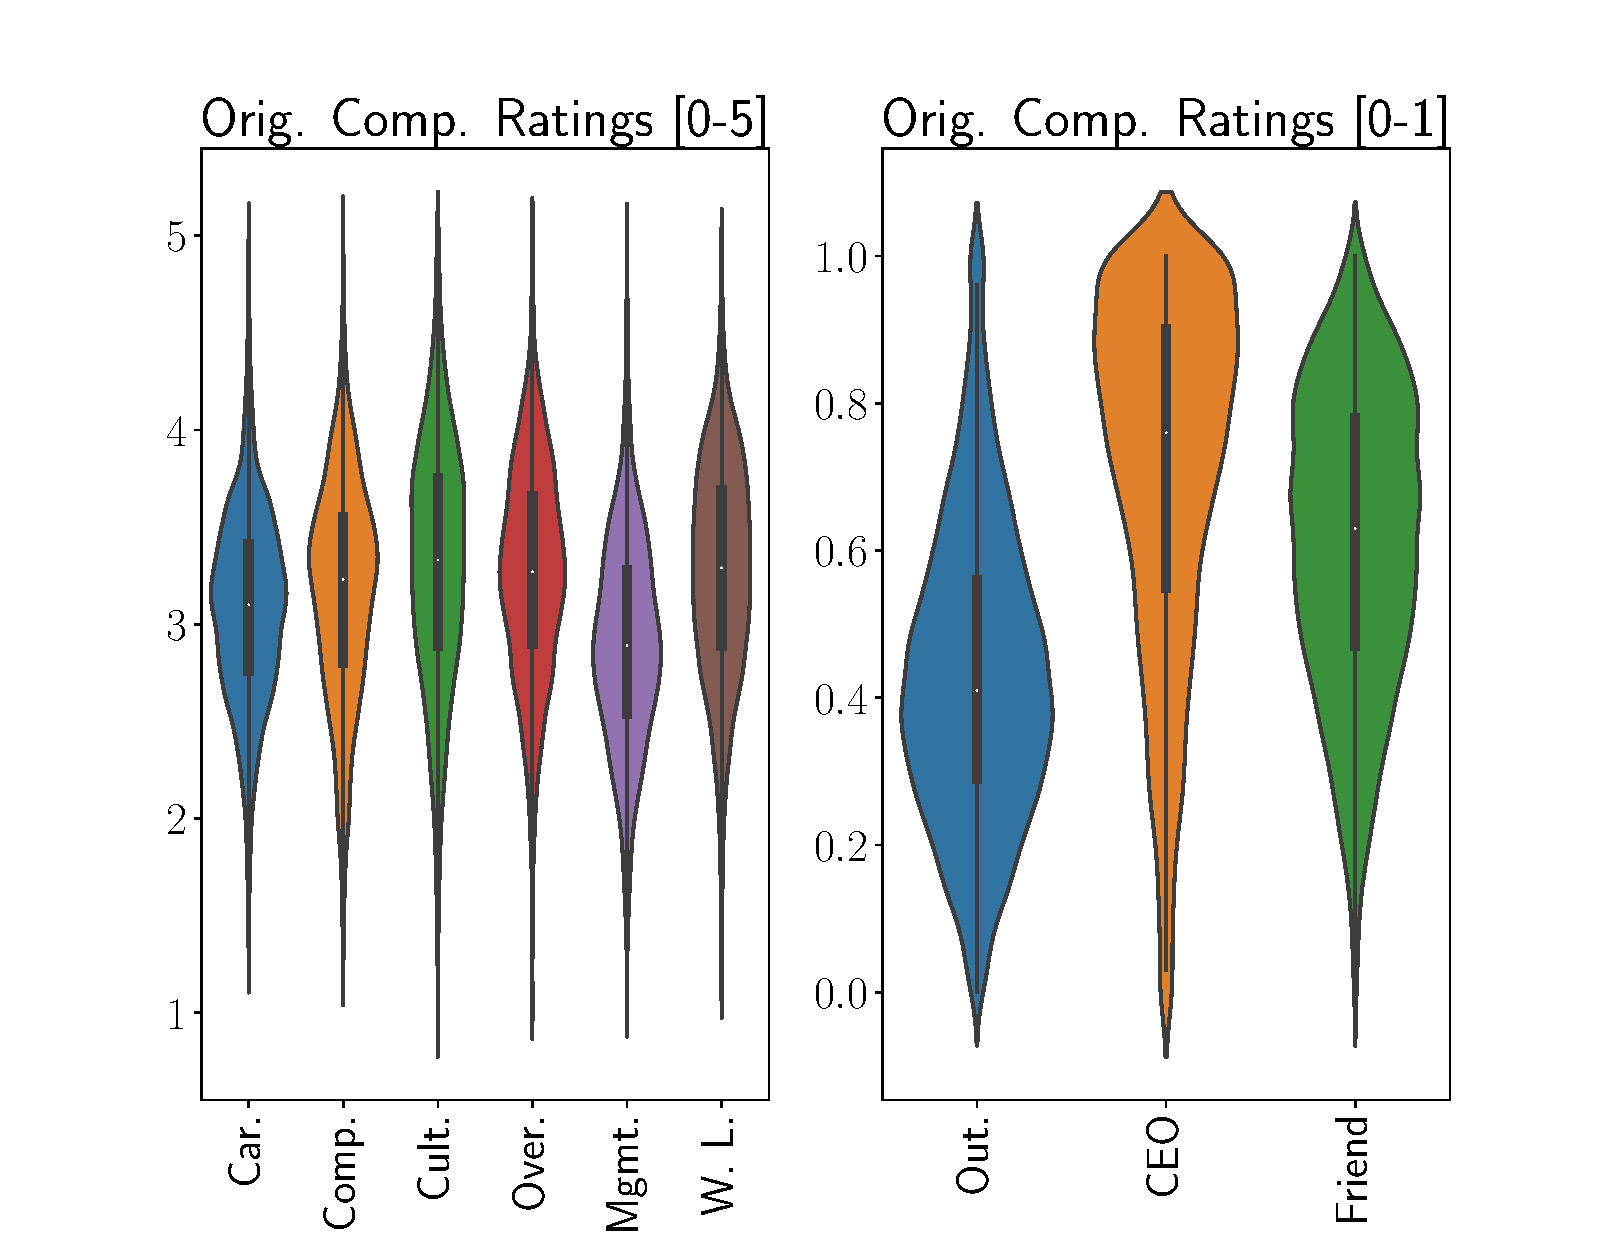
\includegraphics[width=1.0\linewidth]{vioplt.pdf}
    %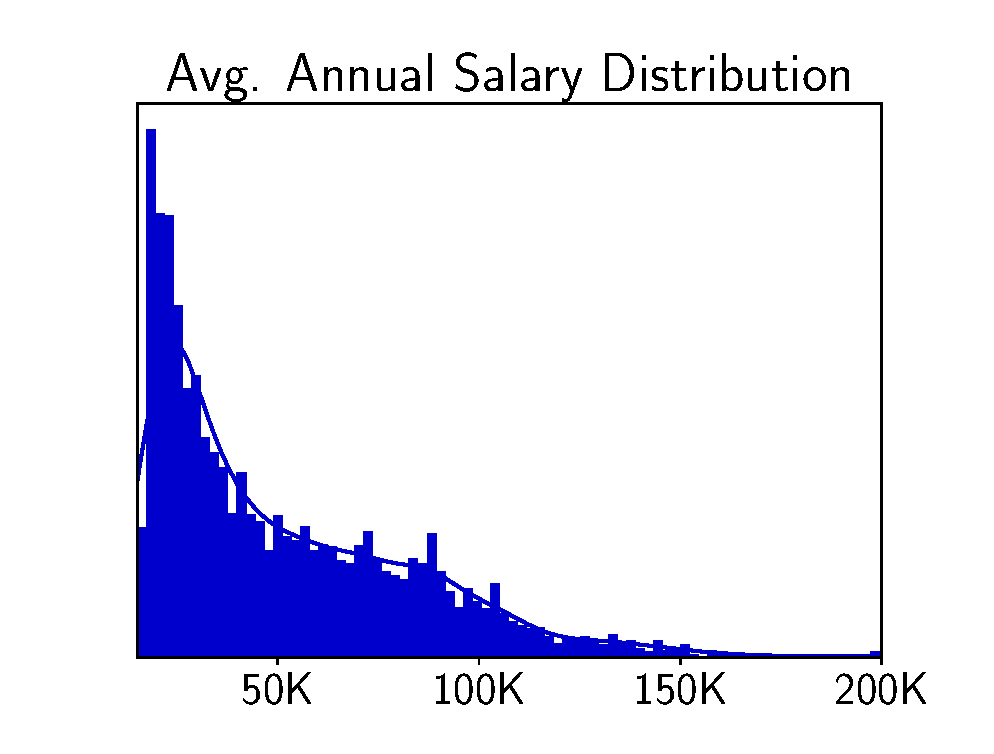
\includegraphics[trim={3cm 3cm 3cm 3cm}, clip,width=0.9\linewidth]{avgsal.eps}
	\caption{Violin plots of original employer ratings information sourced from Glassdoor reviews }
	\label{fig:vioplt}
\end{figure}
%
Ratings with values in the $[0,5]$ range are plotted in the left subplot and those between 
$[0,1]$ range are plotted in the right.  We note that no actual ratings fall outside these 
bounds; the slight graphical extensions beyond these boundaries in the plot are due to 
artifacts of the kernel density estimation procedure required to 
produce the visualization and not representative of the true data. 
In addition note that one can see management ratings tend to be lower overall than 
other related ratings in the left subplot.  In addition, cultural ratings exhibit 
the greatest dispersion, whereas career ratings are comparatively concentrated.
The distribution of $[0,1]$ vary considerably.  In particular, the CEO rating distribution 
is concentrated to the right of the mean largely to a high occurrence of the maximum rating in 
approximately 9\% of the data.  In contrast, company outlook ratings are right-skewed with 
a mean below the average score of 0.5.  Both are less dispersed than the friend recommendation 
rating distribution that also is slightly oriented towards the positive side.

We now describe several elementary features that we construct from the original data that 
will be useful in the below exploratory and predictive studies.  In particular, we will 
consider the percentage salary increase between after a transition has been made. 
In addition, we will consider quantile normalized absolute changes in each rating 
category below, e.g. if an employee moved from a 75\%-tile overall rating employer 
to an 85\%-tile, we will save the 10\%-ile difference as a feature.  We feel these 
features are partially reflect the thought process of an employee who typically leaves an organization 
for higher salary and improved company culture based on the relative rather than absolute 
differences in these variables and thus include them as features.  We finally note that 
all variables are quantile normalized in our predictive model studies so as not to bias 
methods considered due to scaling effects.

\section{Exploratory Insights}

Now we describe a number of findings that were the results of an exploratory analysis of 
the job transition dataset which go beyond the level of summary statistics.  In particular, 
DESCRIBE FINDINGS WHEN FINISHED

\subsection{Transition Salary Changes}
An opportunity to earn a greater salary is often described as a primary motivation 
for a job transition.  We seek to investigate this from a quantitative perspective 
on our attrition dataset.  We first note that approximately 
13\% of transitions occurred without a change in salary. 
In Table \ref{fig:salgr}, we display relative (percentage increase/decrease) and  
absolute salary changes. 
%
\begin{figure}[thb]
    \centering
    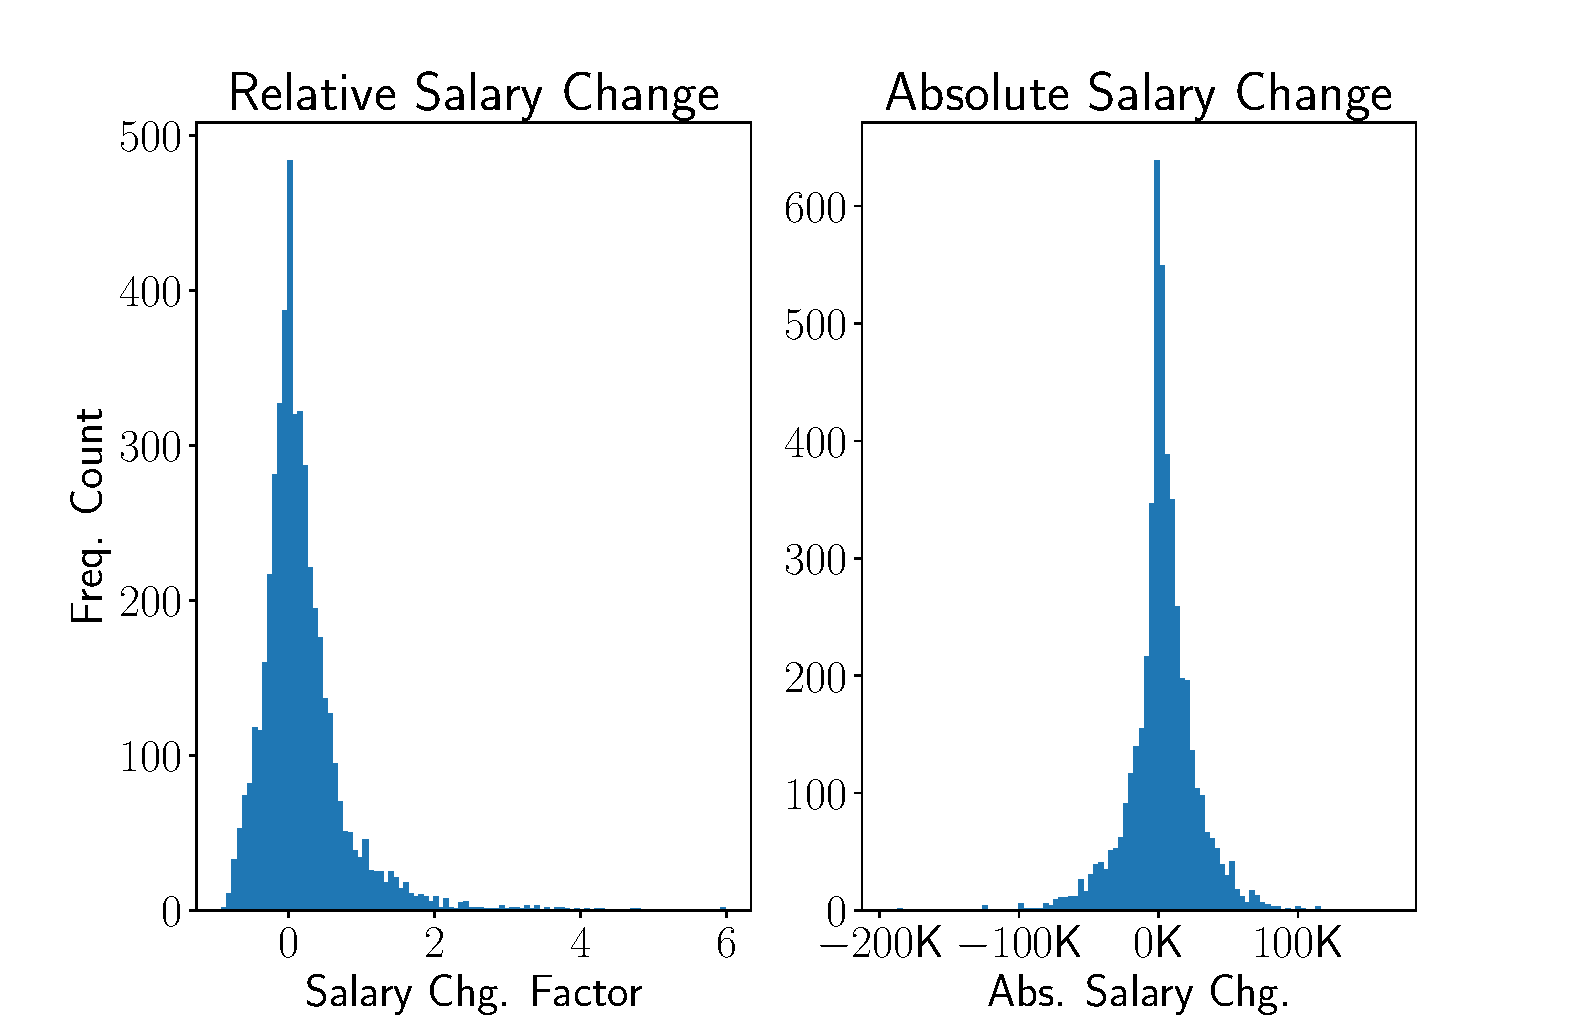
\includegraphics[width=1.0\linewidth]{salgr.pdf}
    %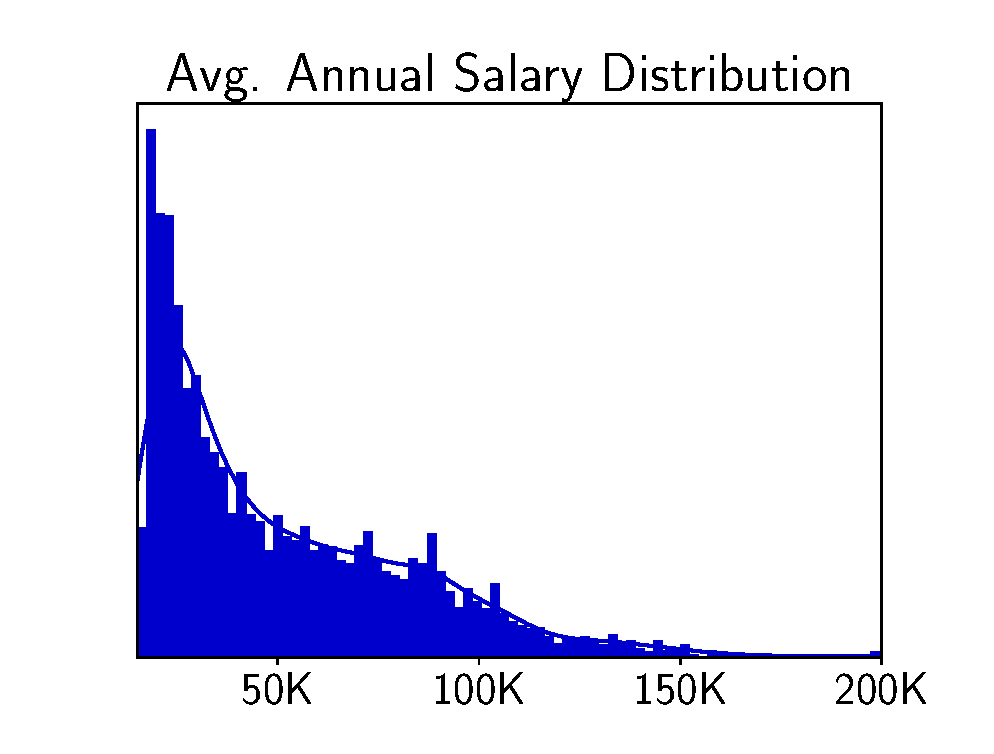
\includegraphics[trim={3cm 3cm 3cm 3cm}, clip,width=0.9\linewidth]{avgsal.eps}
	\caption{Relative and absolute salary differences after a job transition}
	\label{fig:salgr}
\end{figure}
%
First note that this example illustrates the need for considering 
features such as relative change since the asymmetry of the relative change salary distribution is 
prominent whereas this is not as clear in the absolute change plot.  
Second, note that there is a wide range of magnitudes of relative salary changes.  In particular, 
approximately 5\% of employees received a salary increase of more than 150\%.  In 
addition, 36\% took a reduction in salary as a part of their transition.  However, the remainder 
received a salary increase which was in many cases quite substantial. 

In the extreme case, one employee transitioned from a teaching assistant to 
education Director at Michigan State University and received approximately a 6X 
salary increase.  In the opposite direction, one employee transitioned from a \$230,000 
salary as a Managing Director in the Education industry to a Logistics coordinator 
with a \$43,600 annual salary. 

\subsection{Industry Transition Patterns}

Next, we examine how employers either choose to move to a new industry or remain
in that of their origination firm as a consequence of their job transition.  
In Figure \ref{fig:transmat}, we display a heatmap of the percentage of 
employees that started in an industry indicated by the left row labels and 
transitioned into the industry on the lower column label. 
%
\begin{figure}[thb]
    \centering
	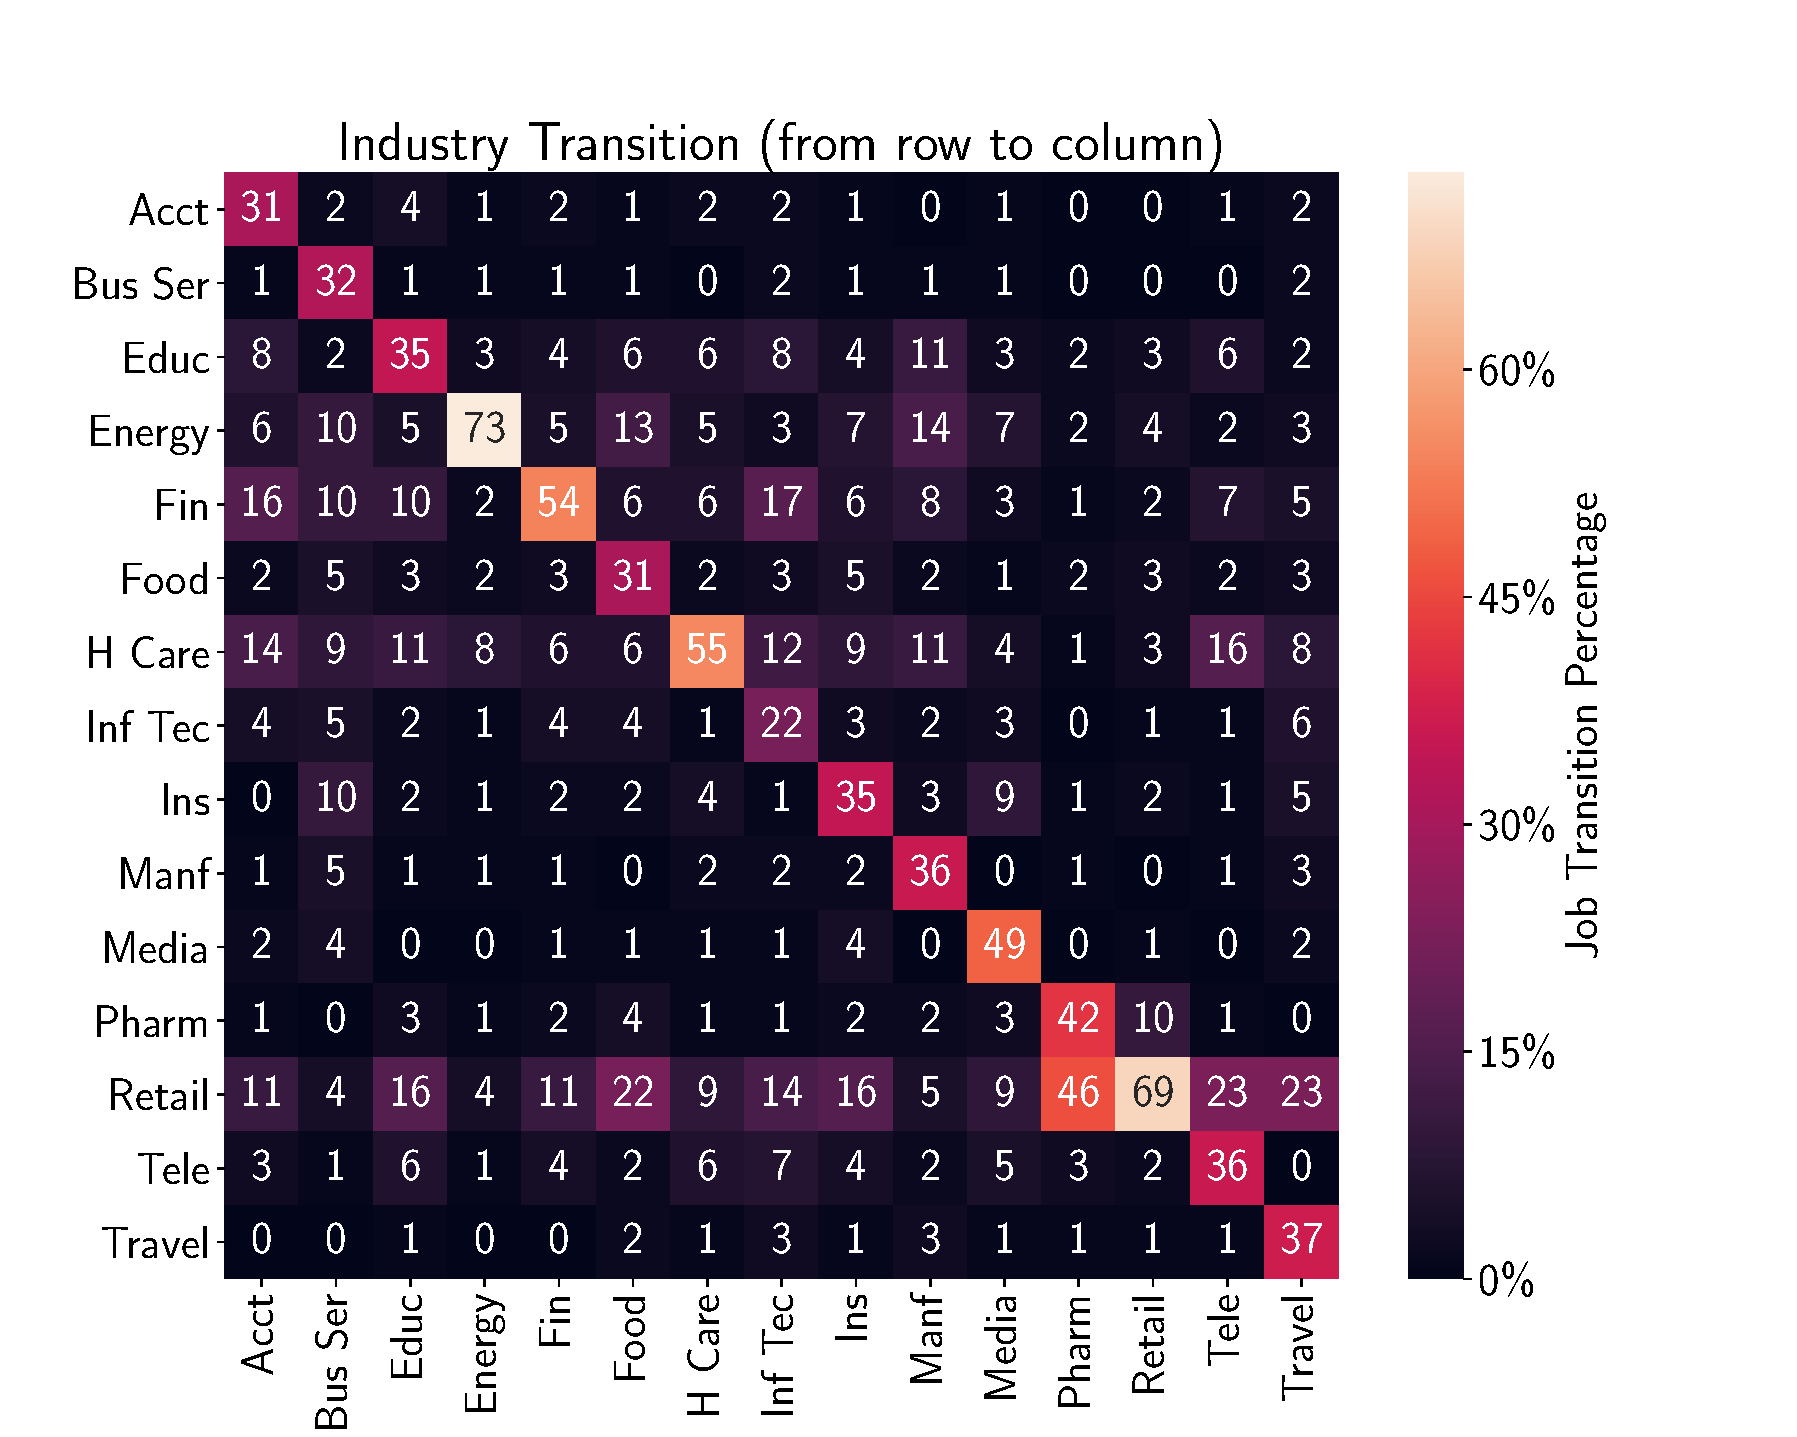
\includegraphics[width=1.0\linewidth]{transmat.pdf}
    %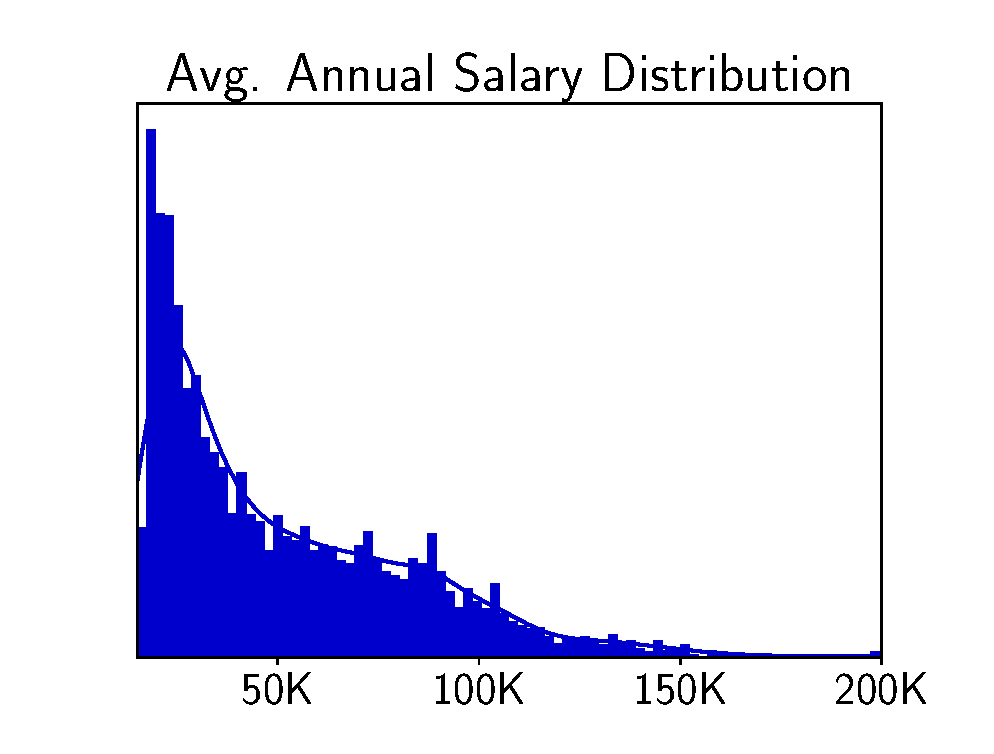
\includegraphics[trim={3cm 3cm 3cm 3cm}, clip,width=0.9\linewidth]{avgsal.eps}
	\caption{Industry transition percentage: original firm 
   industry given in columns and new/same in rows}
	\label{fig:transmat}
\end{figure}
%
Note that both the energy and retail industries tend to retain a considerably 
greater portion of their employees than the others.  An interesting example 
along these lines is the Pharmaceutical industry of which 46\% of employees 
transition to the retail industry while only 42\% remain; this is the only industry 
that exhibits that feature.  Moreover, the information technology industry has 
the lowest retention rate with more than half of transitions out of this industry 
going to the financial, health care, retail, and education sectors.  This is understandable 
due to the skill requirements prevalence of IT positions across all these industries.  
Finally, we note that the retail industry is the most popular industry to transition 
into overall from a distinct original sector.

\subsection{Attrition Identification Variable Importance}

Now, we separate out attrition dataset into the group of job transitions 
where employees remained with their current employer, and those who 
choose to find a new employer. We compared the distributions of all 
numerical variables available in this dataset for both groups 
in order to identify which variables has the most distinct 
distributions.  In Figure \ref{fig:discdist}, we display the 
distributions the original firm friend recommendation and 
worklife balance rating variables for employees who 
stayed with their original firm (green) or transition to a new one (red). 
%
\begin{figure}[thb]
    \centering
	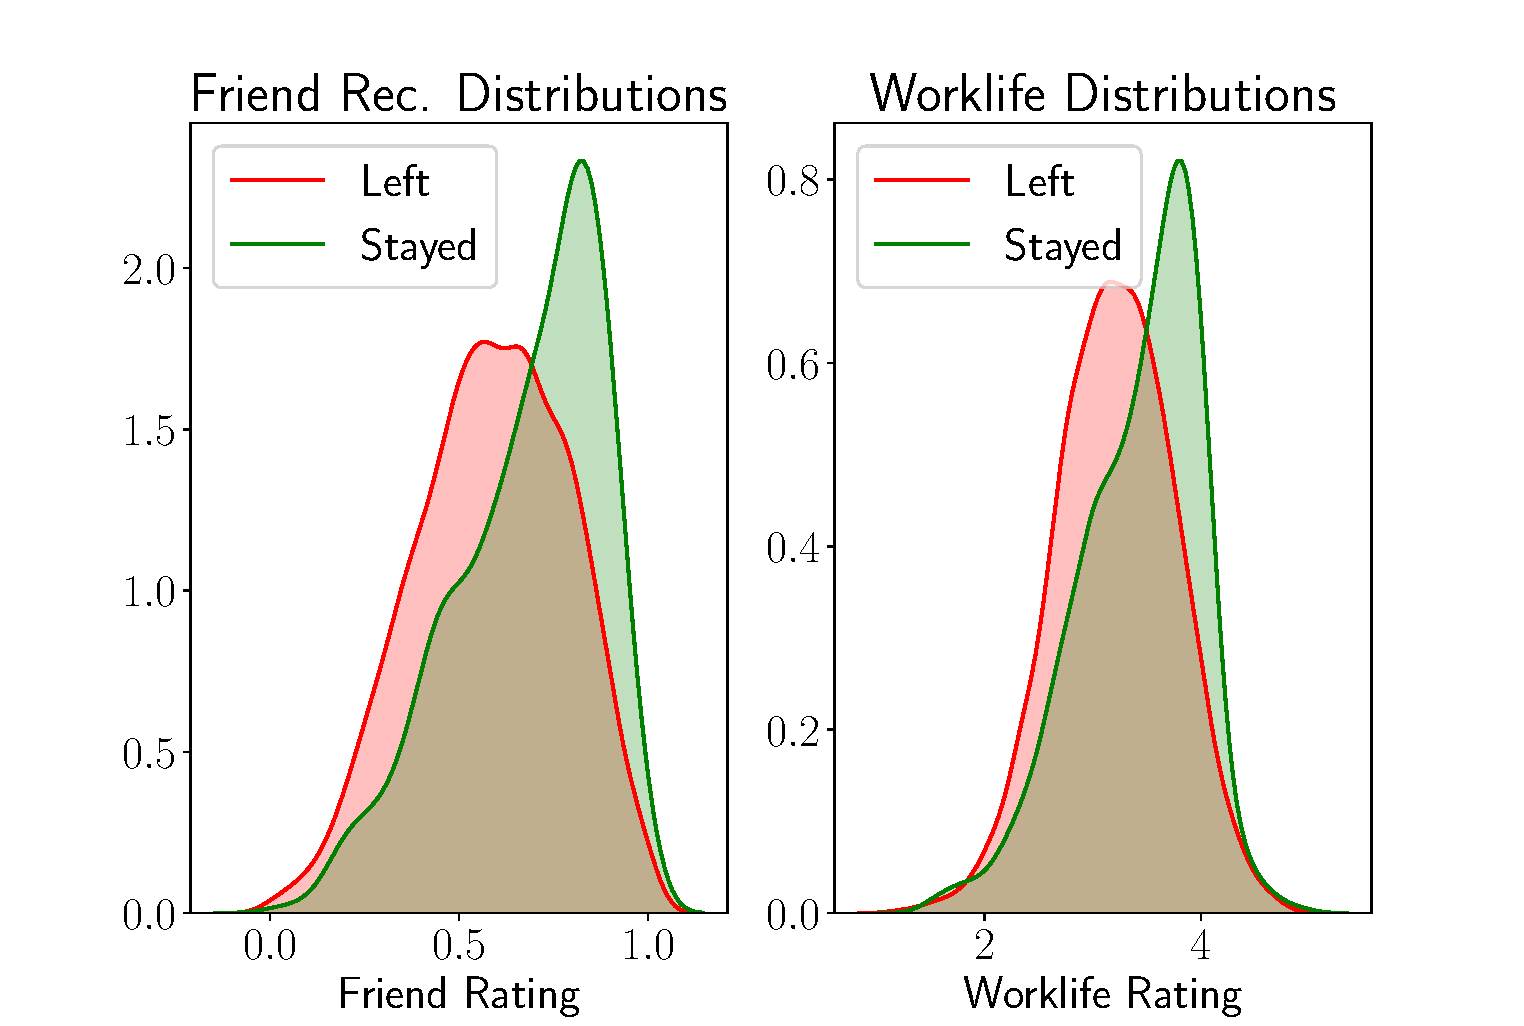
\includegraphics[width=1.0\linewidth]{discdist.pdf}
    %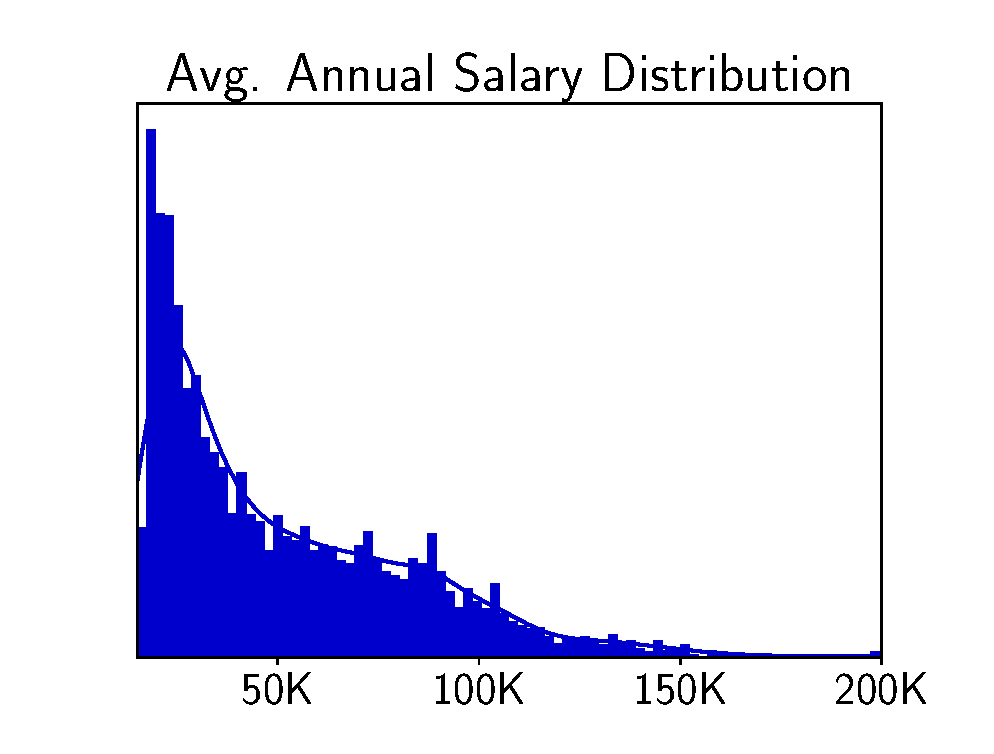
\includegraphics[trim={3cm 3cm 3cm 3cm}, clip,width=0.9\linewidth]{avgsal.eps}
	\caption{Friend recommendation and worklife rating distribution for internal 
    and external transitions}
	\label{fig:discdist}
\end{figure}
%
In addition, we note that the cultural rating distributions exhibited a similar 
although less pronounced behavior.  This provides an indication that both 
these variables will be of importance when attempting to discriminate between 
the two groups in our latter predictive studies. 

\subsection{Firm Ratings Principal Components}

When users fill out Glassdoor surveys that ultimately determine the 
company ratings provided in the attrition dataset, they are asked to 
rate a firm in the nine categories described in Section \ref{datdes}.
It is natural to allows one's overall view on the firm influence 
the manner in which ratings are assigned for each of these
categories, i.e. they are not necessarily independent.  We will 
conduct a principal component analysis on a quantile normalized 
version the our full original ratings dataset of nine categories in 
order to ascertain the effective dimensionality of this information. 

Specifically, let $r_i^j$ for $i=1,\ldots,n=5550$ and $j=1,\ldots,9$ denote 
the $i$ ratings available for category $j$. Consider the sample covariance 
estimator of the quantile normalized ratings data
%
\begin{equation}
    \hat{\Sigma} = \frac{1}{n-1}\sum_{i=1}^n (r_i^j-\bar{r}^j)(r_i^j-\bar{r}^j)^T. 
\end{equation}
%
where here $\bar{r}^j$ denotes the mean value of the $j$-th variable.  Then, we 
perform an eigen-decomposition 
%
\begin{equation}
    \hat{\Sigma} = Q\Lambda Q^{-1}
\end{equation}
%
where here the $i$-th vector of $Q$ is the $i$-th eigenvector of $\hat{\Sigma}$ with 
corresponding eigenvalue $\lambda_i$ which is the $(i,i)$ entry of the diagonal matrix 
$\Lambda$.  This decomposition holds since $\hat{\Sigma}$ is assumed to be positive 
definition, and addition, we take an ordering $\lambda_1\geq\lambda_2\geq \ldots\geq \lambda_9$,
c.f. \cite{Shlens05atutorial} for an overview of principal component analysis.

In Figure, \ref{fig:pcagr}, in the left subplot we display a heatmap of the 
original employer ranking correlation matrix.  Note that all such values 
are generally ranking variables are highly correlated which demonstrates 
that it is necessary to account for the dependency structure of the ranking 
variables.  In the left subplot, we display the percentage variance explained curve 
whose values are defined to be $w_i = \sum_{j=1}^i\lambda_i/\sum_{j=1}^9\lambda_j$. 
%
\begin{figure}[thb]
    \centering
	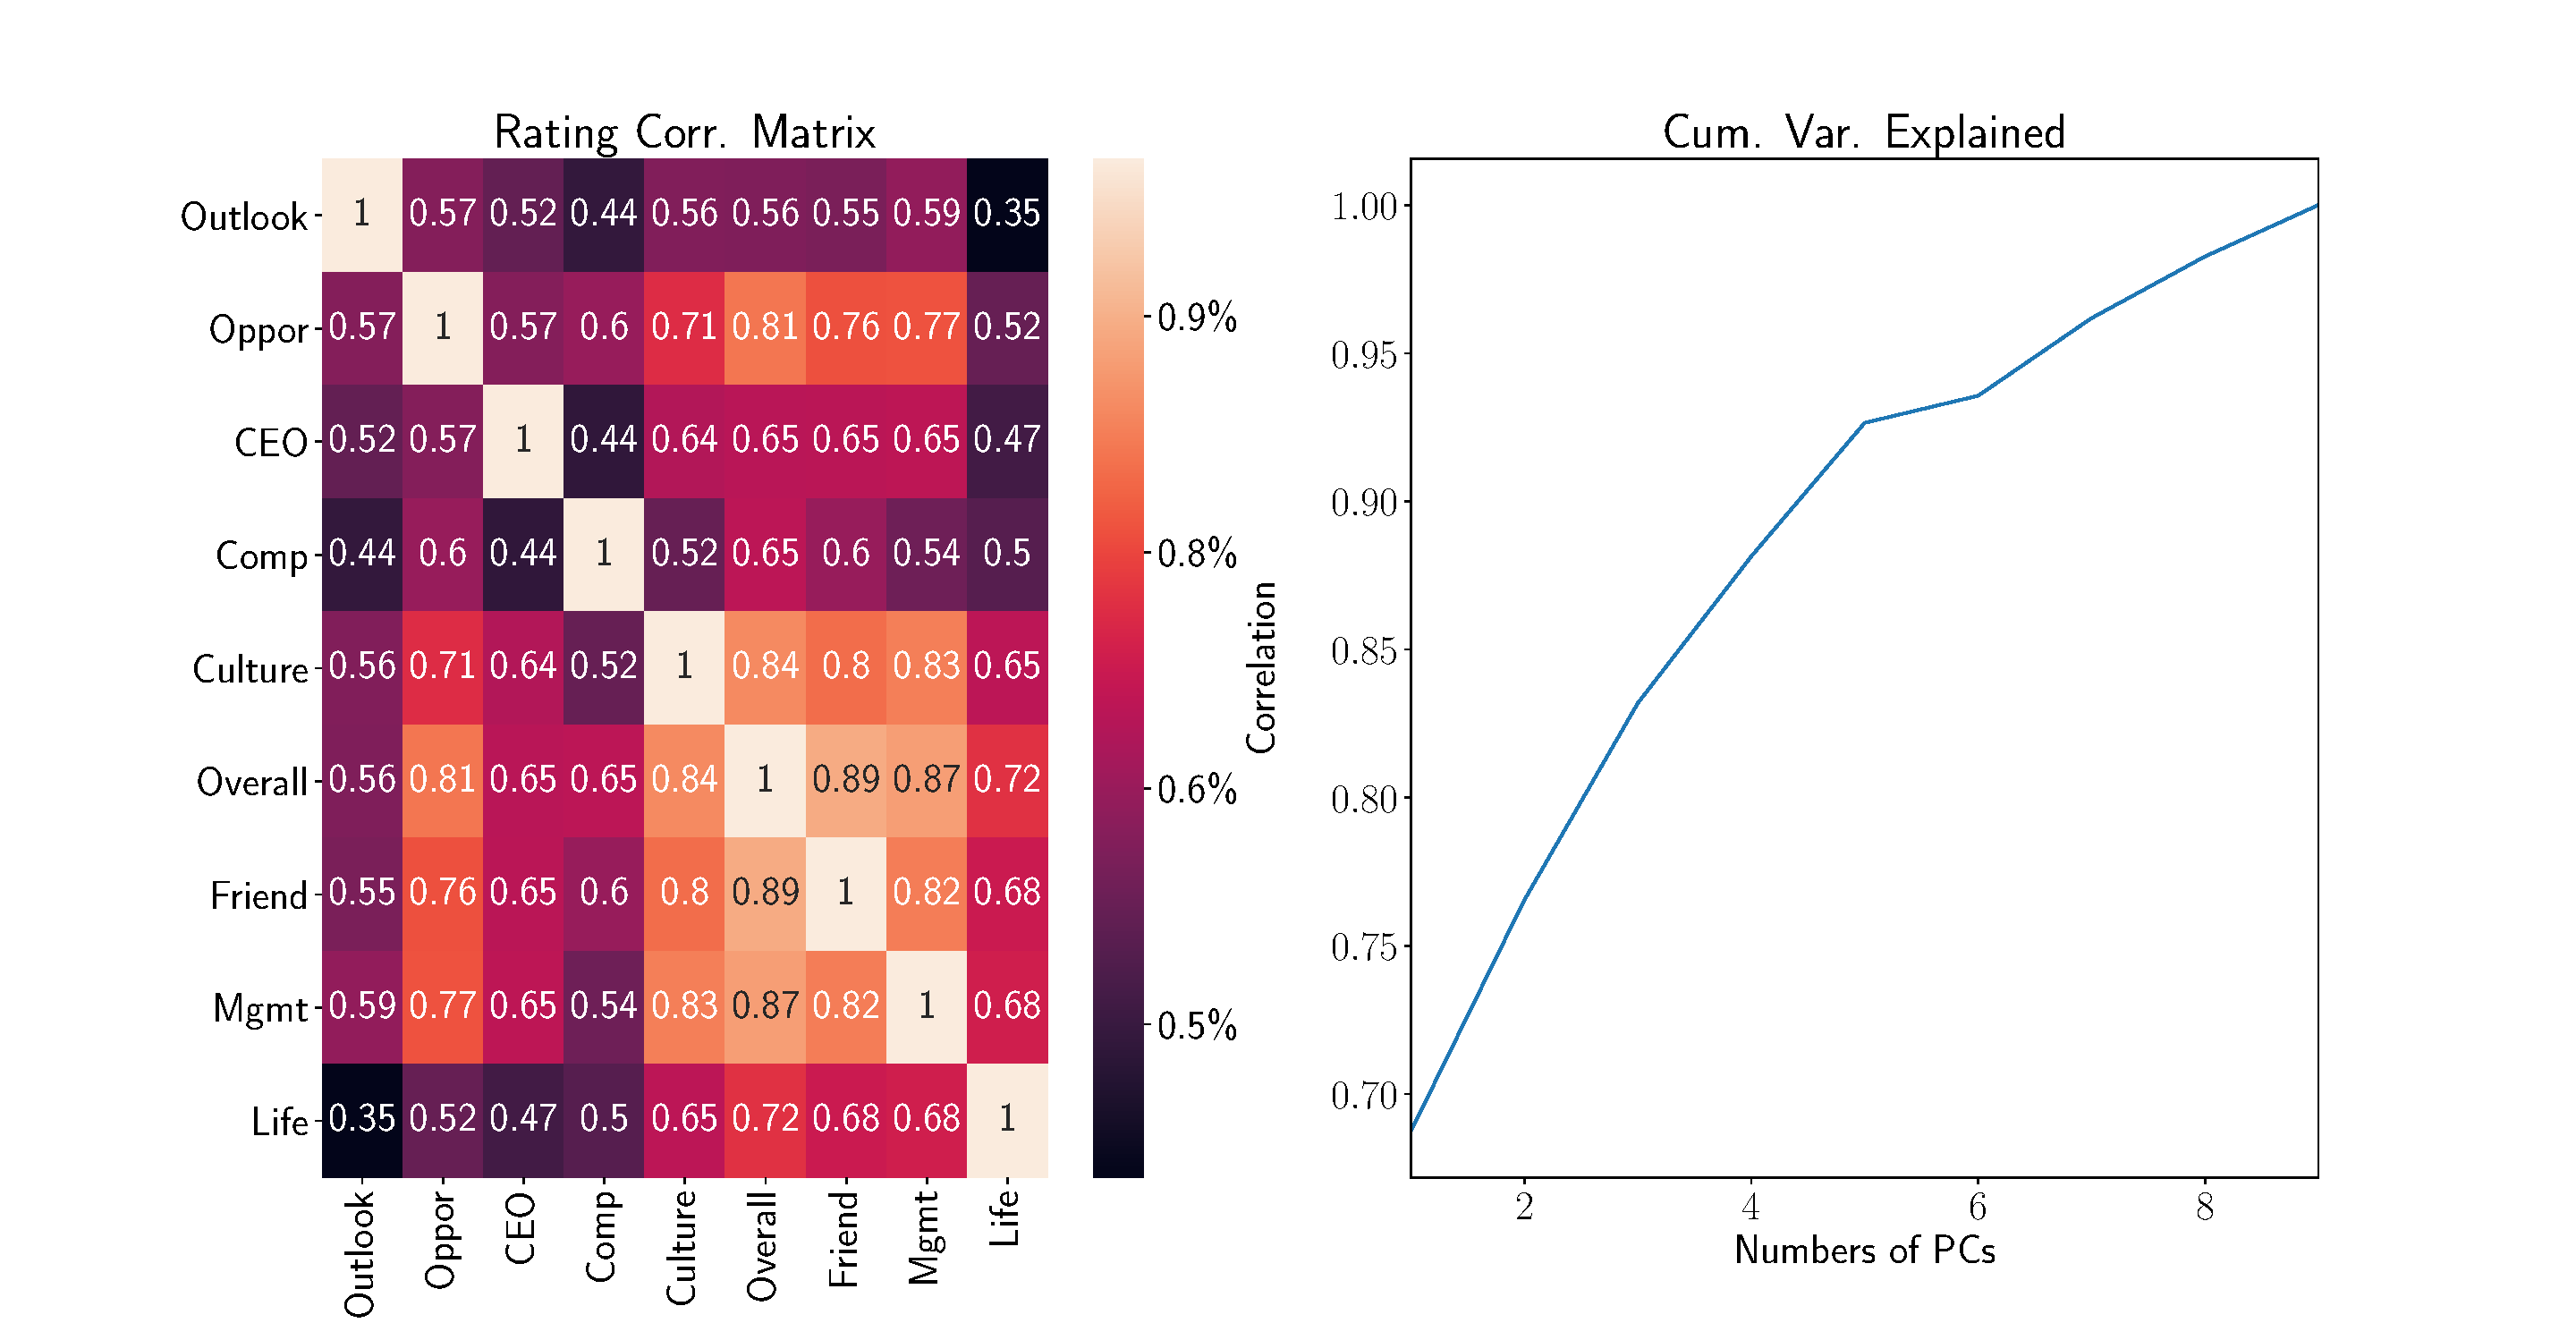
\includegraphics[width=1.0\linewidth]{pcagr.pdf}
    %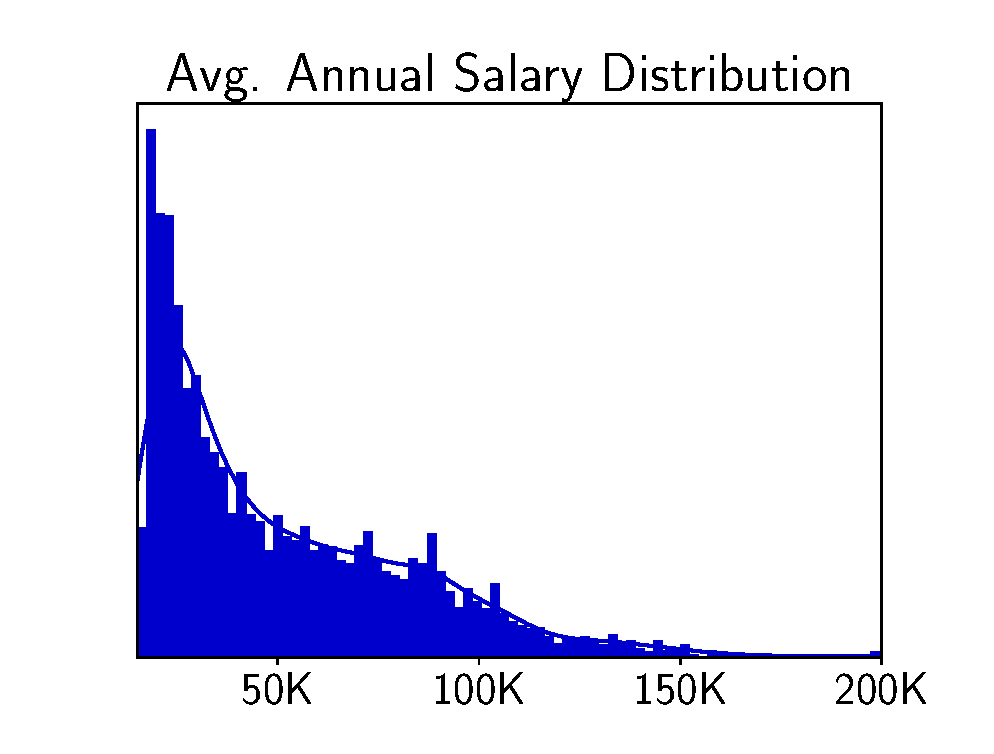
\includegraphics[trim={3cm 3cm 3cm 3cm}, clip,width=0.9\linewidth]{avgsal.eps}
	\caption{Original employer ranking correlation matrix and percentage variance 
    explained curve}
	\label{fig:pcagr}
\end{figure}
%
The first principal component contains just under 70\% of the variation of the data 
and is given in normalized form by  
%
\begin{equation}
    q_1 = [0.27,0.34,0.30,0.28,0.36,0.38,0.37,0.37,0.30] 
\end{equation}
%
which is near a uniform weighted average of the rankings with additional 
weight placed on career opportunities, overall, and friend recommendation, 
senior management rankings. In addition the percentage variance explained 
gradually increases to approximately 92\% at five principal components and 
there is no clear separation between the signal and noise portions of this data.
We conclude that it will be useful to include the quantile normalized 
ranking weighted average in our subsequent predictive studies, but we 
also retain all ratings variables given these percentage variance explained results. 

\subsection{Idea 5: THINK OF IDEA}


\section{Towards an Attrition Model}

adf

Our aim is now extend beyond exploratory data analysis and systematically construct 
a model to predict whether an employee will remain with their original employer or 
leave for another firm during a job transition.

\subsection{Linear Review}


\subsection{Logistic Work}


\subsection{Binary Classifier}

\subsection{Model Performance Comparison}

\section{Conclusions and Extensions}


Here we describe several ideas to pursue as part of this study

Mention limitations here (same as in glassdoor article and others that we find) ... then 
mention that our extensions will overcome these limitations 

-- company specific analytics
-- competative analysis
-- linkedin, full glassdoor dataset 
-- outlier determination may serve as a glassdoor fake review filter 


% For one-column wide figures use
%\begin{figure}[thb]
	% Use the relevant command to insert your figure file.
	% For example, with the graphicx package use
%    \centering
%	
\includegraphics[trim={3cm 3cm 3cm 3cm}, clip,width=0.9\linewidth]{sample-image}
	% figure caption is below the figure
%	\caption{Sample figure with caption.}
%	\label{fig: sample-figure}       % Give a unique label
%\end{figure}

\textbf{Acknowledgements:} The authors would like to ack... for sharing data FINISH WHEN DONE

% if added before the last page, this command can help balancing columns
%\addtolength{\textheight}{-.2cm} 

%Bibliography 
\bibliographystyle{ieeetr}
\bibliography{sample}

\begin{enumerate}
    \item how does salary increase compare with internal vs external transition? 
    \item Founding date vs tenure
    \item Let's focus on Leaving a company, not just different role in same company 
    %\item Look at rankings from old company to new one; what can we say overall about 
    %     the characteristics of these companies?  What factors did we see the most signi
    %     change in? Make scatter plots/hists here 
    \item job title transition? progression ... Markov chain? 
    \item What other summary statistics are relevant that go beyond what is already in 
          the Glassdoor article? 
    \item Do a brief literature review.  What has been done in this area already?
          Summarize Glassdoor as part of this ... describe the uniqueness of this dataset. 
          Mention it would be of interest to expand ... mine LinkedIn as well to do a 
          more thorough study later. 
    \item do reasons vary by length of job??? 
    \item Look at people who made a major change (e.g. shifted geographic regions. ... more than 500 miles 
          away ... is motivation any different for these people?)
    \item Look at how old vs new ranking variable scatter plots differ from the y=x line, 
        e.g. if employees change, which variables to we find also change significantly?  
          Do some change always in the upwards direction? Linear reg. essentially tries 
          to understand to what extent is this line differs from 1, e.g. if it is 1 for 
          a given variable, then this variable has no influence ... can we develop a 
          better variable influence measure here? 
    \item Look at people who switched industries ... any different motivation here? 
    \item One interesting feature is that employees seldom seem to stay at a company that has the 
          same size as their old one.  Lots of shirts from large to small or vice versa.  Perhaps 
          make this more quantitative? 
    \item  check if job-len corresponds to start,end date difference 
    \item Any info associated with geographic studies?  Large vs small cities? 
    \item  patterns that stem from either age or employment tenure? 
    \item binary model classifer, ROC curve etc. 
    \item impl their original regression model ... test 
    \item  industry specific studies 
    \item Distribution of dates that changes were made ... do we see a pattern on times of the 
          year that moves occurred 
    \item explore patterns between old and new firms using year founded 
\end{enumerate}

\end{document}


\end{document}
